\documentclass[suppldata]{interact}

\usepackage{epstopdf}% To incorporate .eps illustrations using PDFLaTeX, etc.
\usepackage[caption=false]{subfig}% Support for small, `sub' figures and tables

%\usepackage[nolists,tablesfirst]{endfloat}% To `separate' figures tables from text if required
%\usepackage[doublespacing]{setspace}% To produce a `double spaced' document if required
%\setlength\parindent{24pt}% To increase paragraph indentation when line spacing is doubled

\usepackage{soul}
\usepackage{amsmath,amssymb} 
\usepackage{multicol}

\theoremstyle{plain}
\newtheorem{theorem}{Theorem}[section]
\newtheorem{lemma}[theorem]{Lemma}
\newtheorem{corollary}[theorem]{Corollary}
\newtheorem{proposition}[theorem]{Proposition}
\theoremstyle{definition}
\newtheorem{definition}[theorem]{Definition}
\newtheorem{example}[theorem]{Example}
\theoremstyle{remark}
\newtheorem{remark}{Remark}
\newtheorem{notation}{Notation}

\usepackage[natbibapa,nodoi]{apacite}
\setlength\bibhang{12pt}
\renewcommand\bibliographytypesize{\fontsize{10}{12}\selectfont}


\usepackage[pdftex,colorlinks=true,urlcolor=blue,citecolor=black,anchorcolor=black,linkcolor=black]{hyperref}
\usepackage{xcolor}
\usepackage{algorithm} 
\usepackage{algorithmic} 
\renewcommand{\algorithmicrequire}{ \textbf{Input:}}
\setlength{\marginparwidth}{2cm}
\usepackage{todonotes}
\usepackage{lscape}

%%%%%%%%%%%%%%		Breakable Algorithm		%%%%%%%%%%%%%%%%%%%%%%
\makeatletter
\newenvironment{breakablealgorithm}
{% \begin{breakablealgorithm}
	\begin{center}
		\refstepcounter{algorithm}% New algorithm
		\hrule height.8pt depth0pt \kern2pt% \@fs@pre for \@fs@ruled
		\renewcommand{\caption}[2][\relax]{% Make a new \caption
			{\raggedright\textbf{\ALG@name~\thealgorithm} ##2\par}%
			\ifx\relax##1\relax % #1 is \relax
			\addcontentsline{loa}{algorithm}{\protect\numberline{\thealgorithm}##2}%
			\else % #1 is not \relax
			\addcontentsline{loa}{algorithm}{\protect\numberline{\thealgorithm}##1}%
			\fi
			\kern2pt\hrule\kern2pt
		}
	}{% \end{breakablealgorithm}
		\kern2pt\hrule\relax% \@fs@post for \@fs@ruled
	\end{center}
}
\makeatother
%%%%%%%%%%%%%%		Breakable Algorithm		%%%%%%%%%%%%%%%%%%%%%%

%\usepackage[affil-it]{authblk}
%\renewcommand\Authfont{\fontsize{10}{14.4}\selectfont}
%\renewcommand\Affilfont{\fontsize{8}{10.8}\itshape}

\begin{document}

\author{\name{Mengyi Zhang\textsuperscript{a}\thanks{CONTACT Mengyi Zhang. Email: mengyi.zhang@polimi.it}, Arianna Alfieri\textsuperscript{b}, Andrea Matta\textsuperscript{a}}
\medskip
\affil{\small \textsuperscript{a} Department of Mechanical Engineering, Politecnico di Milano, via La Masa 1, 20156 Milano, Italy}
\affil{\small \textsuperscript{b} Department of Management and Industrial Engineering, Politecnico di Torino, Corso Duca degli Abruzzi 24, 10129 Turin, Italy}}


\title{\Large Generation of Mathematical Programming Representation for Discrete Event Simulation Models of Timed Petri Nets}

\maketitle

\bigskip
\begin{abstract}
This work proposes a mathematical programming (MP) representation of discrete event simulation of timed Petri nets (TPN). Currently, mathematical programming techniques are not widely applied to optimize discrete event systems due to the difficulty of formulating models capable to %catch 
correctly represent the system dynamics. This work connects the two fruitful research fields, mathematical programming and timed Petri nets. In the MP formalism, the decision variables of the model %are composed of 
correspond to the transition firing times and the markings of the TPN, whereas the constraints represent the state transition logic and temporal sequences among events. The MP model and a simulation run of the TPN are then totally equivalent, which is validated %with several cases. 
through several applications. Using a TPN model as input, the MP model can be routinely generated and used as white box for further %analysis 
tasks such as sensitivity analysis, cut generation in optimization procedures, and proof of formal properties.


%It is a new formalism of discrete event systems. The MPR-DES is the foundation of developing white-box simulation optimization algorithms. The decision variables of the MPR are the transition firing times and the markings, and the constraints represent the transition firings. The equivalence of the solution of the proposed mathematical programming model and the simulation run using the same sample paths is validated with several cases. The MPR generation has been coded in an automatic procedure that only requires the user to input the timed Petri net model.
\end{abstract}

\begin{keywords}
discrete event simulation, mathematical programming, timed Petri net
\end{keywords}


\section{Introduction}

Discrete event dynamic systems (DEVS) have wide application in manufacturing and service applications. Even though many theoretical and analytical studies on discrete event dynamic systems have been developed, performance of real systems with high degree of complexity can be, sometimes, only evaluated with discrete event simulation (DES). Hence, simulation--optimization algorithms are widely used when numerical performance evaluation must be coupled with optimization, i.e., when the best system configuration, according to some criteria, has to be found meanwhile guaranteeing a given value of some performance measures \citep{fu20115book}.  

Most of the simulation--optimization studies consider DES as a \textit{black--box} function. Under the black--box setting, simulation and optimization modules are %decoupled, except that simulation module needs to provide the performance measures of certain solutions when the optimization module queries. With quite limited information from simulation, the optimization module must have many trials, so the black--box procedure can be computationally inefficient.
decoupled. The simulation module provides the performance measure of a given solution generated by the optimization module, which can help a further optimization round. However, the information given by simulation in a black--box setting is quite limited. Hence, the optimization module is almost blind and cannot be very effective, which leads to possibly many trials. This is the main cause for large computational inefficiencies of the overall black--box procedure.

A promising direction to improve the %inefficiency 
efficiency of black--box procedure is to merge the system dynamics into optimization, i.e., considering DES as \textit{white--box} and modeling system dynamics as part of mathematical programming (MP) models. Several works studying such issue can be found in the literature. To cite a few examples, an MP model was proposed to minimize the makespan of single--server manufacturing systems in \citep{di2020makespan}, the buffer allocation problem in multi--stage production flow lines with blocking is addressed in \citep{matta2008simulation}, \citep{weiss2015buffer} and \citep{alfieri2020time}, the optimization of multi stage systems with complex blocking mechanisms are studied in \citep{pedrielli2015integrated}. Decomposition or linear approximation approaches are applied to solve the MP models, %and it can be rather efficient than black-box algorithms and the optimality is also enhanced 
which improve the efficiency of black--box algorithms, thus enhancing also optimality \citep{weiss2015buffer}\citep{alfieri2020time}. 


However, white--box simulation--optimization approaches are not as widely--applied as black--box ones. The reason is that developing a white--box algorithm requires %one 
to master discrete event dynamic systems, %its
simulation and mathematical programming, %but those
and these disciplines are not tightly connected. The above mentioned works are all tailored to specific cases, and there is a lack of generalization to extend %the works 
them to other problems. To fill this gap, this work proposes an approach to translate the simulation of a timed Petri net (TPN) into MP models.


In the literature, a few works address similar problems, i.e.,  translating the behavior of general discrete event dynamic systems into mathematical programming representation. \cite{bemporad1999control} proposed a mixed integer programming modeling framework for hybrid systems, whose states are mixed integer, in discrete time. Differently, this work deals with continuous--time discrete--state systems. \cite{chan2008optimization} proposed a modeling framework to translate a DES model into an MP model starting from an Event Relationship Graph (ERG) representation of the system dynamics. However, despite its generality the ERG representation is not as commonly--used as TPNs. Indeed, developing an ERG model is time consuming and %and the 
as a consequence their approach is not used often. On the other hand, TPNs are well--known representations taught in most engineering study courses, and software tools for easy creation of TPN models also exist. 


The benefits of using MP models to represent discrete event systems are many. As already mentioned, %above,
when coupled with optimization, the MP-based algorithms can be faster and %gain 
reach better solution than black--box optimization algorithms. Furthermore, black--box approaches have limited capability in solving constrained optimization problems, %but 
while MP--based approaches can easily deal with them \citep{zhang2020models}. The vast theoretical and methodological results developed in the MP field can be introduced into the study of DEVS through simulation. For instance, using sensitivity analysis of MP models, gradient estimates can be easily derived as suggested in \citep{chan2008optimization}. In fact, %we do not proposed 
this paper does not propose to totally replace simulation with MP, but to enrich the toolbox for analyzing and optimizing DEVS. Finally, the application of MP models of DEVS is not limited to optimization but also to show formal properties of the system under study. For instance, \cite{basile2012k} proposed the sufficient and necessary condition of K-diagnosability of TPN based on MP analysis. 


The major concern about the application of MP is the computational complexity, %and the solving procedure
as the solution procedure can be time--consuming or even unbearable. However, many approaches from optimization community are available to improve the efficiency. Linear programming approximation \citep{alfieri2012mathematical}, Benders decomposition \citep{weiss2015buffer}, row--column generation \citep{alfieri2020time}, have been studied to solve optimization problems in %reality
real contexts based on mathematical programming representation of DEVS.


The contribution of this work is to propose the first framework translating TPNs into MP models. The translation procedure can be conveniently implemented in general--purpose programming languages and turned into an automated procedure. This work lays a foundation %of 
for developing MP--based approaches %for analyzing and optimizing 
that can be used to analyze and optimize TPNs, based on the vast literature available in the mathematical programming field. 
%The proposed MP models can also be easily transformed into an MPR for optimizing the design parameters of the DES, which are common optimization problems in operations management field.  


The rest of the paper is organized as follows. Section \ref{sec:sim} briefly introduces the TPN and its simulation algorithm. Section \ref{sec:TPN_MPR} describes the generation of the MP model from an existing TPN model. Section \ref{sec:example} shows examples of application and validation of the equivalence between simulation and the MP. Discussion and conclusion are reported in Section \ref{sec:conclude}.



%alternating simulation and optimization procedures, thus, possibly leading to computational inefficiency if the number of iterations and/or the computation time per iteration increases too much. 

% On the contrary, a minority of the simulation--optimization literature explores the structure of the DES models, and such approaches are referred to as \textit{white--box} simulation--optimization. 



%The benefit of white--box simulation--optimization is the saving of simulation budget or computation time since the optimization procedure is guided by the information contained in the structure of the DES model (\cite{zhang2020sample}). However, the barrier to the use of white--box simulation--optimization is modeling DES as white box, so that it eventually favors optimization. 


%The benefit of developing an MPR might be not obvious (especially when there is already a DES model) due to the extremely high complexity of solving it. 
%One may be confused about the motivation of this work, i.e., why one wants the MPR when he/she has already a simulation model at hand, since the complexity of solving mathematical programming is usually high. 
%However, this work does not suggest solving the MPR directly with state-of-the-art optimizers. Instead, the optimal solution of the MPR can be obtained from a simulation run. The added value of the MPR is that the structure of the DES can be explored. With the vast theoretical and methodological results developed in the mathematical programming (MP) field, for instance sensitivity analysis as suggested by \cite{chan2008optimization}, the MPR of a simulation model favors the optimal design and control of the discrete event systems. 

%This work proposes a procedure to establish a white--box simulation model, which is an equivalent Mathematical Programming Representation (MPR) model, based on the well-known event--scheduling logic (\cite{law2014simulation}) applied to timed Petri net (TPN). %for  
%The procedure is applicable to certain types of DES models, and the assumptions that the DES model should satisfy are also presented in this work.
%Specifically, the modeling procedure, the assumptions which the DES model has to satisfy so that it can be applied and some examples are discussed. 

%In this work, we present how to establish an equivalent Mathematical Programming Representation (MPR) of Discrete Event Simulation (DES). The MPR depicts the dynamics of an event-scheduling approach of simulation modeling with a certain sample path. To develop the MPR, state variables, events, initial state, termination condition and the samples of the random variate should be provided. All requirement is also essential each time an event-scheduling algorithm is programmed. Furthermore, the proposed approach is quite routined. Thus, no extra knowledge or skills are required when one has the event-scheduling simulation implementation and wants to apply our approach. Besides the modeling approach, we provide the conditions to check before applying our approach, and discuss what the modifications can be done when some conditions are violated. Some examples are also given.

%Considering the literature on simulation--optimization, 
%\cite{chan2008optimization} proposed a modeling framework to translate a DES model into an MPR model in a general sense. Their modeling framework is based on the Event Relationship Graph (ERG) of the system dynamics. To derive the MPR, % model, 
%an ERG of the DES must be constructed and expanded to an elementary ERG (EERG) model, and a procedure can be applied to translate the EERG model into an MPR. %model. 
%However, this procedure has some limitations. First, deriving an ERG is not an easy task, and the user must pay quite much attention to detect all the event relationships and complete the triggering conditions between each pair of related events. %That 
%The difficulty of developing ERG limits the wide spread of this procedure. Second, the modeling procedure is case--by--case depending on the event relationships, which means that the user must analyze the event relationships one by one and identify which type of modeling, including the variables and constraints, he/she should apply for each event relationship. Consequently, an automatic procedure was not proposed. 
%which means the user has to first identify which situations he/she faces by analyzing the relationships between each couple of events in the EERG, and then choose the appropriate model, including the variables and constraints. 
%This is quite %a burden
%difficult, since EERG is an expansion of ERG; the resulting graph could be huge and writing down the complete MPR model could be even impossible. 



%The automatic MPR generation procedure can be easily implemented in a general-purpose programming language. 
%Despite 
%being different, the MPRs proposed in this work and \cite{chan2008optimization} lead to 
%equivalent results, which, in turn, are both equivalent to a simulation realization.


%Many works in literature show the potentiality of this research direction. For instance, the gradient can be conveniently estimated from the simulation model, if the MPR is approximated into Linear Programming (LP) and %solving 
%the dual can be conveniently obtained (\cite{chan2008optimization}). Moreover, if some of the parameters in the MPR are changed to decision variables, the MPR becomes an integrated simulation--optimization model. Solving the integrated model provides the optimal solution of the optimization problem (\cite{matta2008simulation}). MP--based algorithms, such as linear programming approximation (\cite{alfieri2012mathematical}), Benders decomposition (\cite{weiss2015buffer}), row-column generation (\cite{alfieri2020time}), have been applied to improve the efficiency of %solving the 
%integrated MP model solution. 


%The application of MPR--based simulation--optimization approaches is usually found in operations management of manufacturing and service systems. %The integrated simulation--optimization model has proved itself to be well suited in solving the buffer allocation problem \citep{zhang2020BAP}. %The most efficient approach to finding the sample--path global optimal of the buffer allocation problem of serial production line is developed based on it \citep{zhang2020BAP}. 
%Thanks to the flexibility of DES in evaluating complex systems, the buffer allocation problem of production systems with complex blocking mechanism, such as kanban control, base stock control, extended kanban control, can be managed \citep{pedrielli2015integrated}. Thanks to the flexibility of MPR in modeling optimization problems, problems involving real--valued decision variables such as optimal production rate \citep{tan2015mathematical}, bottleneck detection and throughput improvement problem \citep{zhang2020models} have all been well addressed and the sample--path global optimal solution can be obtained. %It is worthy to notice that, 
%The flexibility of DES for complex system evaluation and of MPR for modeling optimization problems, allowed the integrated simulation-optimization approach to be effectively applied to buffer allocation problems (\cite{zhang2020BAP}), even with complex blocking mechanisms (\cite{pedrielli2015integrated}) and to problems involving real value decision variables (\cite{tan2015mathematical,zhang2020models}). 
%Before the above-mentioned works were proposed, there were many state--of--the--art heuristic approaches addressing those problems, but without any guarantee of global or local optimality. Thus, the development of MPR--based simulation--optimization has made its contribution in the research area of manufacturing and service system optimization.

%To extend the application of the MPR-based simulation optimization approaches, there is a need of modeling approach to translating DES into MPR under general settings.



\section{Timed Petri Nets} \label{sec:sim}

\subsection{Basic definitions and notations}
A TPN is a directed bipartite graph. The set of nodes in that graph is partitioned into a set of \textit{places} $P$ and a set of \textit{transitions} $T$. Places and transitions are connected with weighted and directed edges. In the example shown in the right side of Figure \ref{fig:gg1_petri}, places (i.e., $p_1$, $p_2$, $p_3$), transitions (i.e., $t_1$, $t_2$) and tokens are represented by white circles, rectangles and small black circles, respectively. Places hold \textit{tokens}, and tokens are transferred through transition \textit{firings}, i.e., one transition firing absorbs tokens from some places and releases them to some other places. Each transition $t\in{T}$ can absorb tokens from all of its precedents, and the number of tokens absorbed from place $p\in P$ is equal to the weight of the edge connecting $p$ and $t$. The number of tokens in each place must be non--negative at any time; hence, a firing of transition $t$ is enabled if and only if the number of tokens in all its precedents $p$ is not smaller than the weight on edge $(p,t)$. Each transition $t\in{T}$ can release tokens to all of its successors, and the number of tokens released to place $p\in P$ is equal to the weight of the edge connecting $t$ and $p$.  It is not necessary that the set of precedents and the set of successors are mutually exclusive. 
\begin{figure}[h]
	\centering
	
\includegraphics[width=0.8\textwidth]{Figures/GG1_petri.png}
	\caption{G/G/2 queue and its TPN model.}
	\label{fig:gg1_petri}
\end{figure}
In a TPN, the duration between the moment of absorption and the moment of release is not always negligible, and the duration is called \textit{firing time}. This work considers firing time %non-negative and that
that are non--negative and can follow arbitrary stochastic distribution. 

The distribution of tokens in the places is called \textit{markings}. The initial state of the system, i.e., the state at time zero, is represented by \textit{the initial marking}. 

Formally, a TPN can be defined as a 6--tuple $N=(P, T, F,W, M_0, \tau)$, where ${P}$ denotes the set of places, ${T}$ denotes the set of transitions, ${F}\subseteq(P\times T)\cup(T\times P)$ denotes the set of edges, $W:F \rightarrow \mathbb{Z}^{+}$ denotes the weights on edges, $M_0:P\rightarrow \mathbb{N}$ denotes the initial marking,
	$\tau:T\rightarrow random\ distribution$ denotes the firing time of transitions.


The illustrative example showed in Figure \ref{fig:gg1_petri} is a G/G/2 queue, in which customers arrive at the queue following an arbitrary arrival process. One of the two identical servers (or the idle one if only one is idle) processes customers in the queue one by one, and the processing time is arbitrarily distributed. After processing, the customer will be immediately released from the system, and the server becomes idle. On the right side of Figure \ref{fig:gg1_petri}, the TPN graph of the G/G/2 system is %presented. 
reported. A token in place $p_1$ shows that it is possible to schedule the arrival of the next customer, and the firing time of transition $t_1$ is equal to the inter-arrival time. At the finish of firing $t_1$, a customer arrives, and it is possible to schedule the next arrival, thus, it releases one token to $p_1$. Furthermore, an arrival will increase the length of the queue by 1, which is represented by the number of tokens in place $p_2$. Two tokens in place $p_3$ shows that two servers are idle. The firing of transition $t_2$ shows the processing of a customer, and it is enabled if and only if at least one server is idle and there is a customer in the queue. Once the process of the customer finishes, i.e., the finish of firing $t_2$, a server is released, and a token is sent to place $p_3$.


\subsection{Simulation of Timed Petri Nets}\label{sec:ModelSim}
The event-scheduling approach is the logic behind all the major DES software and used by practitioners when developing simulation codes with general purpose languages \citep{law2014simulation}. For sake of completeness, the logic for simulating TPN is briefly described in this section. This description will also be useful in the next section to better point out the consistency of the generated MP models with the system dynamics. 

Within the event scheduling worldview of discrete event simulation \citep{zeigler2018theory}, an event is first scheduled and occurs afterwards. 
An \textit{event list} stores all the scheduled events that will occur in the future. The event with the earliest occurring time is polled to occur from the event list, and the clock is advanced to its occurring time. The system state is changed upon the event occurrence, and the new state enables the schedule of new events. A new cycle starts from polling the earliest event. In TPN, events, whose occurrence changes the system state instantaneously, are either start or finish of transition firings in a TPN, since they are the only moments when the marking is changed. Thus, an event in a simulation realization of TPN can be represented by a triple $(t,type,time)$, where $t$ is a transition, $type$ is either \textit{start} or \textit{finish}, and $time$ is the occurring time. 

Given a TPN $N=(P, T, F,W, M_0, \tau)$, its simulation can be implemented as in Algorithm \ref{chtp6:Algo:SimulatePetriNet}. 
\begin{algorithm}
	\caption{Simulating a TPN.}
	\begin{algorithmic}[1]
		\label{chtp6:Algo:SimulatePetriNet}
		\REQUIRE ~~ \\
		Initial markings: $M_0$. \\
		
		\STATE \textbf{Initialization:}
		\STATE \textit{EventList} = \{\}; simulation clock: \textit{clock} $\leftarrow$ 0; current markings: $M\leftarrow M_0$;
		\STATE iteration counter: $k\leftarrow0$.\\
		
		\WHILE{stopping condition is not true}
		\FOR{each transition $t_{1}\in T$}
		\WHILE{current marking enables the firing of $t_1$, i.e., $M(p_{1})\ge W(p_1,t_{1}),\ \forall (p_1,t_{1})\in F$}
		%\STATE \textbf{Start to fire the enabled transition.}
		%\STATE Add event $e_{1}=(t^{'},start,clock,i^{t^{'},start})$ to set $V$, add arc $(\hat{e},e_1)$ to the set $A$; $i^{t^{'},start}\leftarrow i^{t^{'},start}+1$. 
		%\STATE Among the precedent places of $t^{'}$, find the place $p$ such that $(t,p),(p,t^{'})\in F$, if $\bigg( \left \lceil \frac{W(p,t^{'})i-(\bar{x}^p+1)}{W(t,p)} \right\rceil - \left \lceil \frac{W(p,t^{'})i-\bar{x}^p}{W(t,p)} \right\rceil  \bigg)$ is not equal to zero, add arc $(\hat{e},e_1)$ to set $\Upsilon^p$.
		\STATE Sample the firing time $\tau_0$ of random variable $\tau(t_1)$
		\FOR{each precedent place $p_1$ of $t_1$}
		\STATE Remove $W(p_1,t_1)$ tokens from $p_1$: $M(p_1) \leftarrow M(p_1)-W(p_1,t_1)$
		\ENDFOR
		%\STATE \textbf{Schedule the end-of-firing event.}
		\STATE Add event $(t_1,finish,clock+\tau_0)$ to event list.
		%\STATE Add event $e_2$ to set $V$, add arc $(e_1,e_2)$ to the set $A$.
		\ENDWHILE
		\ENDFOR
		%\STATE \textbf{Execute the earliset event.}
		\STATE From \textit{EventList}, take the event $(t_2,finish,time)$ with the earliest time. 
		\STATE Advance the clock: $clock\leftarrow time$.
		%\STATE Update $e$ and index: $e\leftarrow(t,end,time,i^{t,end})$, $i^{t,end}\leftarrow i^{t,end}+1$.
		%\STATE Update last occurring event $\hat{e}\leftarrow e$.
		\FOR{each successive place $p_2$ of $t_2$}
		\STATE Add $W(t_2,p_2)$ tokens to $p_2$: $M(p_2) \leftarrow M(p_2)+W(t_2,p_2)$.
		\ENDFOR		
		\STATE Update iteration counter: $k = k+1$
		\ENDWHILE		
	\end{algorithmic}
\end{algorithm}
In Algorithm \ref{chtp6:Algo:SimulatePetriNet}, event list, clock time and system state (i.e., the markings) are initialized as empty, zero and initial markings, respectively. Each iteration is composed of two steps, i.e., to start all the enabled transitions and to finish the firing in the event list with the earliest finishing time. In the first step, if firing of a certain transition $t_1$ is enabled by the current markings, the firing can be started and tokens are immediately removed from precedent places of $t$. In the mean time, the finish of the firing can be scheduled with a delay equal to the firing time, which is a sample $\tau_0$ of random distribution $\tau(t_1)$, and the finish of firing is added to the event list. It can be noticed that the event list contains only finish--of--firing events, since all the start--of--firing events are executed immediately without going into the list. In the second step, the firing with the earliest finish time will be taken from the event list, and the tokens are released to the successive places. 
The iterative procedure stops when a given condition is reached, which is usually %a limit of iteration numbers or clock time. 
a given number of iterations or a value of the clock time.

%Algorithm \ref{chtp6:Algo:SimulatePetriNet} considers a nondeterministic policy, i.e., if multiple transitions are enabled at the same time, they will fire in any order. One can also define the priority among transitions. In this case, in line 4 of Algorithm \ref{chtp6:Algo:SimulatePetriNet}, transitions with higher priority will be visited first. 


\section{Generation of Mathematical Programming Representations} \label{sec:TPN_MPR}

This section introduces the MP models translating the dynamics of the TPN described in Algorithm 1. Such MP models are mathematical programming representations (MPR) of the TPNs under study. Specifically, the time when transition firings start and finish and markings can all be seen (in the MP model) as decision variables. The time when transition $t$ starts to fire for the $i$-th time is denoted by $e^{t,s}_i$, and $e^{t,f}_i$ denotes the time when the fire finishes. Variables $\mathcal{E}_k$ denotes the simulation clock at the beginning of iteration $k$ in Algorithm 1. Variables $e^{t,s}_{i}$, $e^{t,f}_{i}$ and $\mathcal{E}_k$ are all real--valued and non--negative. Variable $m^p_k$ is used to denote the number of tokens in place $p$ at the beginning of iteration $k$ in Algorithm 1. Some binary variables are also used in the MPR, and they will be introduced in the following, during the explanation of the model. 

\subsection{Completion of transitions}

The first group of mathematical relationships, denoted by group--A, are the constraints for firing %finishes, 
finishing as in lines 14 and 15 of Algorithm 1. 

First of all, sets $\mathbb{K}$, $\mathbb{T}$ and $\mathbb{I}^t$ are used to indicate the set of iterations, the set of transitions and the set of firings of transition $t$, respectively.
Binary variables $w^{t}_{i,k}$ are introduced to represent that the $i$-th start firing of transition $t$ finishes in iteration $k$. If $w^{t}_{i,k}$  is equal to one, %and 
variable $e^{t,f}_{i}$ is bounded to $\mathcal{E}_k$, as shown in constraints (A1) and (A2). Constraints (A3) state that each firing-finish event executes at most once. Constraints (A4) state that, in each iteration, exactly one firing-finish event is executed. Constraints (A5) implies that the delay between the start and finish of firing transition $t$ is equal to a sample from the random variable $T^{t}$. Constraints (A6) imply that the clock cannot be reversed from iteration $k-1$ to iteration $k$. Constraint (A7) implies that the simulation clock is initialized to zero. The value of $M$ in constraints (A1) and (A2) can be set to a value that is larger than the simulation time span, as it is needed to bound the finishing time of transitions.

\begin{eqnarray}
	e^{t,f}_i-\mathcal{E}_k\ge M(w^{t}_{i,k}-1) & \forall\ t\in\mathbb{T},i\in \mathbb{I}^{t},k\in \mathbb{K}&(A1)\nonumber\\
	\mathcal{E}_k-e^{t,f}_i\ge M(w^{t}_{i,k}-1) & \forall\ t\in\mathbb{T},i\in \mathbb{I}^{t},k\in \mathbb{K}&(A2)\nonumber\\
	\sum_{k\in \mathbb{K}} w^{t}_{i,k} \le 1& \forall\ t\in\mathbb{T},i\in \mathbb{I}^{t}&(A3)\nonumber\\
	\sum_{t\in \mathbb{T}}\sum_{i\in \mathbb{I}^{t}} w^{t}_{i,k} =1&\forall\ k\in \mathbb{K}&(A4)\nonumber\\
	e^{t,f}_{i} - e^{t,s}_{i} = \tau^{t}_{i} & \forall t\in\mathbb{T}, i\in \mathbb{I}^{t}&(A5) \nonumber\\
	\mathcal{E}_{k}-\mathcal{E}_{k-1}\ge 0&\forall\ k\in \mathbb{K}&(A6)\nonumber\\
	\mathcal{E}_0 = 0&&(A7)\nonumber
\end{eqnarray}


\subsection{Start of transitions} \label{sec:MPR_start_Firing}

The second group of constraints, denoted by group--B, depicts the start of transition firing, as in lines 5 to 13 in Algorithm 1. Binary variables $x^{t}_{i,k}$ represent that a fire of transition $t$ starts in iteration $k$ if it is equal to one. Constraints (B1) and (B2) shows that the start firing time is equal to the simulation clock. Also in this case, the value of $M$ can be set to a value that is larger than the simulation time span as it is used to bound the transition firing time.

\begin{eqnarray}
	e^{t,s}_i-\mathcal{E}_{k} \ge M(x^{t}_{i,k}-1)& \forall\ t\in \mathbb{T},k\in \mathbb{K},i\in \mathbb{I}^{t}&(B1)\nonumber\\
	\mathcal{E}_{k} -e^{t,s}_i\ge M(x^{t}_{i,k}-1)&\forall\ t\in \mathbb{T},k\in \mathbb{K},i\in \mathbb{I}^{t}&(B2)\nonumber%\\
	%e^{t,s}_i - e^{t,s}_{i-1} \ge 0&\forall\ t\in \mathbb{T},i\in \mathbb{I}^{t} &(B3)\nonumber
\end{eqnarray}

The condition to start firing transition $t$ is that the tokens in all the precedent places $p$ are above the required level $W^p,t$. Binary variables $z^{t}_{k}$ equal to one represents the condition for transition $t$ is true, as constraints (B3). Moreover, a set of binary variables $v^{t,p}_k$ is used to verify if the number of tokens in precedent place $p$ is smaller than $W^{p,t}$, as constraints (B4). The value of $M$ can be chosen as the upper bound of marking of place $p$ minus $(W^{p,t}-1)$. Variable $v^{t,p}_k$ is equal to 1, if marking in place $p$ is smaller than $W^{p,t}$. Constraints (B5) assures that $z^{t}_k$ is equal to zero only if at least one precedent place does not contain enough number of tokens. Constraints (B6) show that if $z^{t}_k$ is equal to one, transition $t$ must start to fire in iteration $k$. Constraints (B7) state that at most one firing of any transition starts for each transition.

\begin{eqnarray}
	m^p_k - W^{p,t} \ge W^{p,t}(z^{t}_{k}-1)&\forall\ t\in \mathbb{T},k\in \mathbb{K},p\in \mathbb{P}&(B3)\nonumber\\
	(W^{p,t}-1) - m^p_k \ge M(v^{t,p}_k-1) & \forall\ t\in \mathbb{T},k\in \mathbb{K},p\in \mathbb{P} &(B4)\nonumber\\
	1 - z^{t}_{k} \le \sum_{p\in \mathbb{P}} v^{p,t}_k&\forall\ t\in \mathbb{T},k\in \mathbb{K}&(B5)\nonumber\\
	\sum_{i\in \mathbb{I}^{t}} x^{t}_{i,k} = z^{t}_k&\forall\ t\in \mathbb{T},k\in \mathbb{K}&(B6)\nonumber\\
	\sum_{k\in \mathbb{K}} x^{t}_{i,k} \le 1& \forall\ t\in \mathbb{T},i\in \mathbb{I}^{t}&(B7)\nonumber
\end{eqnarray}

Constraints (B7) avoid that certain markings can enable firings of the same transition to start multiple times. Thus, modifications are made to the TPN model before the proposed MPR model is applied. The modification is to expand the non--zero--firing-time transition $t$ into two transitions, denoted by $\tilde{t}$ and $\bar{t}$, respectively. Transition $\tilde{t}$ has zero firing time and maintains all the precedent places and their weights of transition $t$, while transition $\bar{t}$ maintains the firing time, successive place and their weights of transition $t$. Transitions $\tilde{t}$ and $\bar{t}$ are both connected to an intermediate place $p_t$, %and 
with one arc %pointed 
directed from $\tilde{t}$ to place $p_t$ and one arc %pointed 
directed from $p_t$ to $\bar{t}$. An example is shown in Figure \ref{fig:tpn_expansion}. This expansion can freeze the simulation clock before all the possible firings of transition $t$ start.

\begin{figure}[h]
	\centering
	
\includegraphics[width=0.8\textwidth]{Figures/TPN_expansion.png}
	\caption{TPN expansion.}
	\label{fig:tpn_expansion}
\end{figure}


\subsection{Event sequencing}
The index $i$ of event $e^{t,s}_i$ represents the sequence of firing starting, i.e., if a firing starts in an earlier iteration, then its index will be smaller. Moreover, a firing must finish after starting. Group--C constraints force such sequences, which are relevant to all the events. Constraints (C1) show that if the $i$--th firing of transition $t$ does not start before simulation termination, then the $(i+1)$--th firing will not start. Constraints (C2) state that if the $i$--th firing of transition $t$ does not start before simulation termination, then it will not finish. Constraints (C3) state that a firing cannot finish before starting, unless it remains in the future event list at the end of the simulation run. Constraints (C4) depict that the $(i+1)$--th firing of transition $t$ must be scheduled after the $i$--th execution, unless the $(i+1)$--th execution is not scheduled before simulation termination. The value of $M$ in constraints (C3) and (C4) can be set to $K$, i.e., the total number of iterations. 

\begin{eqnarray}
	\sum_{k\in \mathbb{K}} x^{t}_{i+1,k} - \sum_{k\in \mathbb{K}} x^{t}_{i,k} \le 0&  \forall\ t\in \mathbb{T},i\in \mathbb{I}^{t}&(C1)\nonumber\\
	\sum_{k\in \mathbb{K}} w^{t}_{i,k}-\sum_{k\in \mathbb{K}} x^{t}_{i,k} \le 0&  \forall\ t\in \mathbb{T},i\in \mathbb{I}^{t}&(C2)\nonumber\\
	\sum_{k\in \mathbb{K}} kw^{t}_{i,k} - \sum_{k\in \mathbb{K}} kx^{t}_{i,k} \ge M(\sum_{k\in \mathbb{K}} w^{t}_{i,k}-1) &\forall\ t\in \mathbb{T}, i\in \mathbb{I}^{t}&(C3) \nonumber\\
	\sum_{k\in \mathbb{K}} kx^{t}_{i+1,k} - \sum_{k\in \mathbb{K}} kx^{t}_{i,k} \ge 1+M(\sum_{k\in \mathbb{K}} x^{t}_{i+1,k}-1)&  \forall\ t\in \mathbb{T},i\in \mathbb{I}^{t}&(C4)\nonumber
\end{eqnarray}

\subsection{State transitions}

The tokens in place $p$ are changed from $m^{p}_{k}$ to $m^{p}_{k+1}$ in iteration $k$, as in constraints (D1) and in lines 16 to 18 in Algorithm 1. The transitions $t$ that start in %fire 
firing in iteration $k$ absorbs $A^{p,t}$ tokens from the precedent places $p$, and the firing that finishes in iteration $k$ releases tokens to the successive places. 

\begin{eqnarray}
	m^p_{k+1} = m^p_k - \sum_{t\in \mathbb{T}} W^{p,t} \sum_{i\in \mathbb{I}^{t}} x^t_{i,k} +  \sum_{t\in \mathbb{T}} W^{t,p} \sum_{i\in \mathbb{I}^{t}} w^t_{i,k} &\forall p\in \mathbb{P}, k\in \mathbb{K}& (D1) \nonumber
\end{eqnarray}

Equation (D1) can also be reformulated as (D2).
\begin{eqnarray}
	m^p_{k+1} = m^p_0 - \sum_{t\in \mathbb{T}} W^{p,t} \sum_{k^{'}=0}^k \sum_{i\in \mathbb{I}^{t}} x^t_{i,k^{'}} +  \sum_{t\in \mathbb{T}} W^{t,p} \sum_{k^{'}=0}^k \sum_{i\in \mathbb{I}^{t}} w^t_{i,k^{'}} &\forall p\in \mathbb{P}, k\in \mathbb{K}& (D2) \nonumber
\end{eqnarray}

\subsection{Objective function}\label{sec:TPN_obj}
With the constraints defined in the previous sections, there is a unique feasible solution in terms of transition firing times and the %history of simulation clock, 
sequence of simulation clock values, i.e., $e^{t,s}_i$, $e^{t,f}_{i}$ and $\mathcal{E}_k$. Thus, the objective function can be any function of %those
these variables, such as, average system time or average waiting time in queueing systems. Notice that multiple feasible solutions may appear in terms of binary variables, since the sequence of events with identical execution time is not uniquely defined.

The flexibility of the objective function definition is a main difference between the formulation proposed by \cite{chan2008optimization} and the approach proposed in this work, since the objective function of MPR in \cite{chan2008optimization} can be only the sum of all the execution times. The uniqueness of the optimal solution and the flexibility of the objective function formulation is particularly beneficial if one wants to make use of the resulting MPR to solve an optimization problem %concerning
related to the design or the operation of the discrete event system (e.g., %for instance 
the capacity of the queue or the control policy of a manufacturing system), since changing the objective function or adding new constraints to calculate the system performance will not influence the equivalence between the  MPR and a simulation run. %This issue will be discussed in Section 4.


%\section{Indicative examples} 
\section{Examples of MPR generation from TPN}
\label{sec:example}
In this section, the $G/G/m$ is used as a example to generate MPR from TPN. Both the proposed and the state-of-the-art formulation are presented. Finally, also an extended model to optimize the $G/G/m$ queue is stated. 

\subsection{MPR of G/G/m queue}\label{sec:MPR_ggm}
A $G/G/m$ queue is composed by $m$ parallel identical servers. Customers arrive at the queue following an general arrival process. One of the identical idle servers processes customers in the queue one by one, and the processing time  of each customer is generally distributed. After being processed, the customer will be released from the system immediately, and the server becomes idle again. In Figure \ref{fig:tpn_GG2}, the TPN of $G/G/2$ is shown. A token in place $p_{arr}$ shows that it is possible to schedule the arrival of the next customer, and the firing time of transition $t_{arr}$ is equal to the inter-arrival time. At the end of firing of $t_{arr}$, a customer arrives, and it is  then possible to schedule the next arrival, i.e., it releases one token to $p_{arr}$. Furthermore, each arrival will increase the length of the queue by 1, which is represented by the number of tokens in place $p_{queue}$. Two tokens in place $p_{idle}$ shows that two servers are idle. The firing of transition $t_{process}$ represents the processing of a customer, and it is enabled if and only if at least one server is idle and there is at least one customer in the queue. Once the process of the customer finishes, i.e., the end of firing of $t_{process}$, the server is released, and a token is sent to place $p_{idle}$.

\begin{figure}[h]
	\centering
	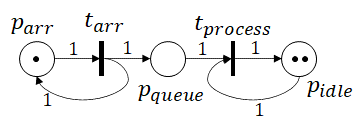
\includegraphics[width=0.45\textwidth]{Figures/TPN-GG2.png}
	\caption{TPN of G/G/2.}
	\label{fig:tpn_GG2}
\end{figure}

As mentioned in Section \ref{sec:MPR_start_Firing}, the transitions with non-zero firing times are expanded before implementing the MPR generation. In the case of G/G/2 queue, transition $t_{process}$ needs to be expanded to $\tilde{t}_{process}$, $\bar{t}_{process}$ and $p_{process}$. Transition $t_{arr}$ does not need expansion since it is self-limiting. The resulting expanded TPN is shown in Figure \ref{fig:tpn_GG2_expansion}.  

\begin{figure}[h]
	\centering
	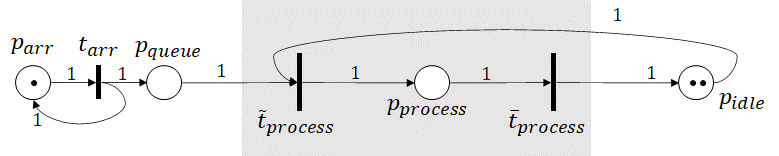
\includegraphics[width=0.8\textwidth]{Figures/TPN-GG2-expansion.png}
	\caption{TPN expansion of G/G/2.}
	\label{fig:tpn_GG2_expansion}
\end{figure}

The sets $\mathbb{T},\ \mathbb{K},\ \mathbb{I}^t$ are specified as follows. Set $\mathbb{T}$ is composed of three transitions $\{t_{arr},\tilde{t}_{process}, \bar{t}_{process}\}$ as shown in Figure \ref{fig:tpn_GG2_expansion}. If $n$ job arrival, processing and departure are simulated, each of the three transitions is fired for $n$ times, and the set $\mathbb{I}^t$ is equal to $\{1,2,..., n\}$. There are $3n$ transition firings in the simulation execution and the set $\mathbb{K}$ is equal to $\{0,1,..., 3n-1\}$. The initial markings $m^{p_{arr}}_0,\ m^{p_{queue}}_0, m^{p_{process}}_0, m^{p_{idle}}$ are specified as 1, 0, 0, 2. Once the TPN with the initial markings and the simulation length are provided, the MPR %composed of 
corresponding to constraints (A1) to (A7), (B1) to (B7), (C1) to (C4) and (D1) can be generated. The implementation pseudo code is presented in Algorithm \ref{Algo:Implementation}. 

\begin{eqnarray}
	\mathbb{T} = \{t_{arr},\tilde{t}_{proc}, \bar{t}_{proc}\} \nonumber\\
	\mathbb{K} = \{0,1,..., 3n-1\} \nonumber\\
	\mathbb{I}^t=\{1,2,..., n\} \nonumber
\end{eqnarray}

\begin{algorithm}
	\caption{Implementation pseudo code.}
	\begin{algorithmic}[1]
		\label{Algo:Implementation}
		\REQUIRE ~~ \\
		Timed Petri net: $N=(\mathbb{P}, \mathbb{T}, F, W, M_0, \tau)$. \\
		Number of firing of each transition $t$: ${I}^t$ and index set $\mathbb{I}^t$\\
		Total number of firings: $K$ and index set $\mathbb{K}=\{0,1,...,K-1\}$\\
		
		\STATE \textbf{Expand TPN:}
		\FOR {transition $t\in\mathbb{T}$:}
			\IF {$t$ has non-zero firing time}
				\STATE Expand $t$ into $\tilde{t}, p_t, \bar{t}$ and update $N$.
			\ENDIF
		\ENDFOR
		
		\FOR{$t\in\mathbb{T}$, $i\in\mathbb{I}^t$, $k\in\mathbb{K}$}
		\STATE (A1), (A2), (B1), (B2)
		\ENDFOR
		
		\FOR{$t\in\mathbb{T}$, $i\in\mathbb{I}^t$}
		\STATE (A3),(A5),(B7),(C1),(C2),(C3),(C4)
		\ENDFOR
		
		\FOR{$k\in\mathbb{K}$}
		\STATE (A4),(A6)
		\ENDFOR
		
		\FOR{$t\in\mathbb{T}$, $k\in\mathbb{K}$, $p\in\mathbb{P}$}
		\STATE (B3),(B4)
		\ENDFOR
		
		\FOR{$t\in\mathbb{T}$, $k\in\mathbb{K}$}
		\STATE (B5),(B6)
		\ENDFOR
		
		\FOR{$p\in\mathbb{P}$, $k\in\mathbb{K}$}
		\STATE (D1),(D2)
		\ENDFOR
	\end{algorithmic}
\end{algorithm}



\noindent
Table \ref{tab:sim_GGM} shows the first ten iteration of a simulation run of a G/G/m queue.

In iteration 0, the system is in its initial state with markings (1,0,0,2), and transition $t_{arr}$ can be fired; equivalently, binary variables $z^{arr}_0$ and $x^{arr}_{1,0}$ are equal to $1$ in the solution of the MPR. The time to start firing transition $t_{arr}$ is equal to $0$, and the variable $e^{arr,s}_{1}$ takes value $0$ in the MPR solution. The fire will finish at time 2.3, and variable $e^{arr,f}_{1}$ takes value 2.3 equivalently. %That firing is also the firing to finish in this iteration, and 
As that firing finished in the current iteration, $w^{arr}_{1,0}$ is equal to 1. After that, the markings are changed to (1,1,0,2) and the current iteration ends. 

At the beginning of iteration 1, the simulation clock is advanced to the time of the firing has finished in iteration 0, i.e., $2.3$. In the MPR solution, the variable $\mathcal{E}_1$ is then equal to $2.3$. With markings (1,1,0,2), it is possible to fire $t^{arr}$ and $\tilde{t}^{proc}$, and variables $z_1^{arr}$ and $z_1^{\tilde{proc}}$ are equal to 1. These firings are the second and first firing of $t^{arr}$ and $\tilde{t}^{proc}$, respectively, and variables $x_{2,1}^{arr}$ and $x_{1,1}^{\tilde{proc}}$ take value 1 in the MPR solution. The starting time of the transitions $t^{arr}$ and $\tilde{t}^{proc}$ are equal to the clock time, and variables $e^{arr,s}_{2}$ and $e^{\tilde{proc},s}_{1}$ are equal to $2.3$. With a sample from the arrival process, the next customer will arrive at time 11.1, i.e., the finishing time of transition $t^{arr}$ is equal to 11.1, which is the value of variable $e^{arr,f}_{2}$. Since transition $\tilde{t}^{proc}$ is zero-firing-time, the firing will finish at time 2.3, which is the value of variable $e^{\tilde{proc},f}_{1}$. There are two firings to be finished in the queue, and that of $\tilde{t}^{proc}$ has earlier time, so it will be the firing that will be finished in this iteration and, hence, variable $w^{\tilde{proc}}_{1,1}$ is equal to one. After that, the markings are changed to $(0,0,1,1)$ and the iteration ends. 

Similarly for iterations 2 to 10, the values of the MPR variables in the solution and the simulation realizations, %can be justified 
which are reported in Table \ref{tab:sim_GGM}, can be explained as done for iterations 0 and 1.
 
\begin{landscape}
	\begin{table}
		\caption{Simulation run and MPR solution of G/G/m queue.}
		\label{tab:sim_GGM}
		\begin{tabular}{llllll}
			\hline
			$k$ & $clock$& Markings & Start firings & Unfinished firings & Finish Firing  \\ \hline
			
			0 &0 & $(1,0,0,2)$& $t^{arr}$ & $t_{arr}:2.3$ & $t_{arr}:2.3$ \\
			&$\mathcal{E}_0=0$   &$\mathbf{m}_0 = (1,0,0,2)$ & $z^{arr}_{0} = 1, x^{arr}_{1,0}=1, e^{arr,s}_{1}=0, e^{arr,f}_{1}=2.3$ & & $w^{arr}_{1,0}=1$ \\ \hline
			
			1 & 2.3 & $(1,1,0,2)$ & $t^{arr},\tilde{t}^{proc}$ & $\tilde{t}_{proc}:2.3, t^{arr}:11.1$ & $\tilde{t}_{proc}:2.3$ \\
			& $\mathcal{E}_1=2.3$ & $\mathbf{m}_1 = (1,1,0,2)$ & $z^{arr}_{1} = 1, x^{arr}_{2,1}=1, e^{arr,s}_{2}=2.3,  e^{arr,f}_{2}=11.1$ & & $w^{\tilde{proc}}_{1,1}=1$ \\ 
			&  &  & $z^{\tilde{proc}}_{1} = 1, x^{\tilde{proc}}_{1,1}=1, e^{\tilde{proc},s}_{1}=2.3, e^{\tilde{proc},f}_{1}=2.3$ & &  \\ \hline
			
			2 & 2.3 & $(0,0,1,1)$ & $\bar{t}_{proc}$ & $\bar{t}_{proc}:6, t^{arr}:11.1$ & $\bar{t}_{proc}:6$ \\
			& $\mathcal{E}_2=2.3$&$\mathbf{m}_2=(0,0,1,1)$&$z^{\bar{proc}}_{2} = 1, x^{\bar{proc}}_{1,2}=1, e^{\bar{proc},s}_{1}=2.3, e^{\bar{proc},f}_{1}=6$ & & $w^{\bar{proc}}_{1,2}=1$ \\ \hline
			
			3 & 6 & $(0,0,0,2)$ & &	 $t^{arr}:11.1$ & $t^{arr}:11.1$\\
			& $\mathcal{E}_3=6$ & $\mathbf{m}_3=(0,0,0,2)$ & & &$w^{arr}_{2,3}=1$ \\ \hline
			
			4 & 11.1 & $(1,1,0,2)$ & $t^{arr}, \tilde{t}^{proc}$ &  $ \tilde{t}^{proc}:11.1, t^{arr}:12.1$ & $\tilde{t}_{proc}:11.1$ \\
			& $\mathcal{E}_4=11.1$ & $\mathbf{m}_4=(1,1,0,2)$ & $z^{arr}_{4} = 1, x^{arr}_{3,4}=1, e^{arr,s}_{3}=11.1,e^{arr,f}_{3}=12.1$ & & $w^{\tilde{proc}}_{2,4}=1, $ \\ 
			&  &  & $z^{\tilde{proc}}_{4} = 1, x^{\tilde{proc}}_{2,4}=1, e^{\tilde{proc},s}_{2}=11.1, e^{\tilde{proc},f}_{2}=11.1$ & &  \\ \hline
			
			5 & 11.1 & $(0,0,1,1)$ & $\bar{t}_{proc}$ & $t^{arr}:12.1, \bar{t}_{proc}:16.9$ & $t^{arr}:12.1$ \\
			& $\mathcal{E}_5=11.1$&$\mathbf{m}_5=(0,0,1,1)$&$z^{\bar{proc}}_{5} = 1, x^{\bar{proc}}_{2,5}=1, e^{\bar{proc},s}_{2}=11.1, e^{\bar{proc},f}_{2}=16.9$ & & $w^{arr}_{3,5}=1$ \\ \hline
			
			6 & 12.1 & $(1,1,0,1)$ & $t^{arr}, \tilde{t}^{proc}$ & $\tilde{t}^{proc}:12.1, t^{arr}:15.2, \bar{t}_{proc}:16.9$ & $\tilde{t}^{proc}:12.1$\\
			& $\mathcal{E}_6=12.1$ & $\mathbf{m}_6=(1,1,0,1)$& $z^{arr}_6=1, x^{arr}_{4,6}=1, e^{arr,s}_{4}=12.1, e^{arr,f}_{4}=15.2$ && $w^{\tilde{proc}}_{3,6}=1$ \\
			&  & & $z^{\tilde{proc}}_6=1, x^{\tilde{proc}}_{3,6}=1, e^{\tilde{proc},s}_{3}=12.1, e^{\tilde{proc},f}_{3}=12.1$ &&  \\ \hline
			
			7 & 12.1 & $(0,0,1,0)$ &$\bar{t}^{proc}$ & $t^{arr}:15.2, \bar{t}^{proc}:16.9, \bar{t}^{proc}:20.1$ & $t^{arr}:15.2$ \\
			&  $\mathcal{E}_7=12.1$ &$\mathbf{m}_7=(0,0,1,0)$ & $z^{\bar{proc}}_{7} = 1, x^{\bar{proc}}_{3,7}=1, e^{\bar{proc},s}_{3}=12.1, e^{\bar{proc},f}_{3}=20.1$ &  & $w^{arr}_{4,7}=1$\\ \hline
			
			8 & 15.2 & $(1,1,0,0)$ &  $t^{arr}$ & $\bar{t}^{proc}:16.9, t^{arr}:17.8, \bar{t}^{proc}:20.1$ & $\bar{t}^{proc}:16.9$\\
			& $\mathcal{E}_8=15.2$ & $\mathbf{m}_8=(1,1,0,0)$& $z^{arr}_{8} = 1, x^{arr}_{5,8}=1, e^{arr,s}_{5}=15.2, e^{arr,f}_{5}=17.8 $ &&$w^{\bar{t}^{proc}}_{2,8}=1$\\ \hline
			
			9 & 16.9 & $(0,1,0,1)$ & $\tilde{t}^{proc}$ & $\tilde{t}^{proc}:16.9, t^{arr}:17.8, \bar{t}^{proc}:20.1$ & $\tilde{t}^{proc}:16.9$\\
			& $\mathcal{E}_9=16.9$ & $\mathbf{m}_9=(0,1,0,1)$ & $z^{\tilde{proc}}_{9} = 1, x^{\tilde{proc}}_{4,9}=1, e^{\tilde{proc},s}_{4}=16.9,  e^{\tilde{proc},f}_{4}=16.9$ &&$w^{\tilde{proc}}_{4,9}=1$\\ \hline
			
			10 & 16.9 & $(0,0,1,0)$ & $\bar{t}^{proc}$ & $t^{arr}:17.8, \bar{t}^{proc}:20.1, \bar{t}^{proc}:25.5$ & $t^{arr}:17.8$\\
			& $\mathcal{E}_{10}=16.9$ & $\mathbf{m}_{10}=(0,0,1,0)$ & $z^{\bar{proc}}_{10} = 1, x^{\bar{proc}}_{4,10}=1, e^{\bar{proc},s}_{4}=16.9,  e^{\bar{proc},f}_{4}=25.5$&&$w^{arr}_{5,10}=1$\\
			
			\hline
		\end{tabular}
	\end{table}
\end{landscape}

\subsection{Comparison with Schruben's model of G/G/m systems}
In \cite{chan2008optimization}, an MPR of DEVS simulation based on ERG is presented. The ERG of the $G/G/2$ queue is shown in Figure \ref{fig:ERG_GG2}. In the ERG, nodes and arcs represent the events and the triggering relationships. The simulation of the $G/G/2$ queue is composed of three events, which are $arrival$, $starting\ process$ and $finishing\ process$, respectively. The three events are presented by nodes $Arr$, $Start\ proc$ and $Fin\ proc$ in the ERG. The node $Run$ indicates the launch of the simulation. There are two state variables for $G/G/2$ queue, $queue$ and $idle$, representing the number of jobs in the queue and the number of idle servers. The equations below each node state how the state variables are changed upon the execution of the events. For instance, when event $Arr$ occurs, one job enters the system and $queue$ is incremented by one. When there is an arc connecting two nodes, it means that it is possible to execute the destination event only after the source event is executed. %under certain conditions. 
The execution of an event can also be subject to certain conditions, reported as labels on the connecting arc. The conditions can be a time delay or a logic expression. %, labeled on the arcs. 
The arc pointing from $Arr$ to $Arr$ is accompanied with a time delay $\tau{arr}$, indicating that the next job will arrive with a time delay equal to the inter-arrival time from the previous one. The arc pointing from $Arr$ to $Start\ proc$ is %accompanied 
labeled with the logic expression $idle\ge 1$, indicating that after a job is arrived, it can start to be processed only if there is at least one idle server.

\begin{figure}[h]
	\centering
	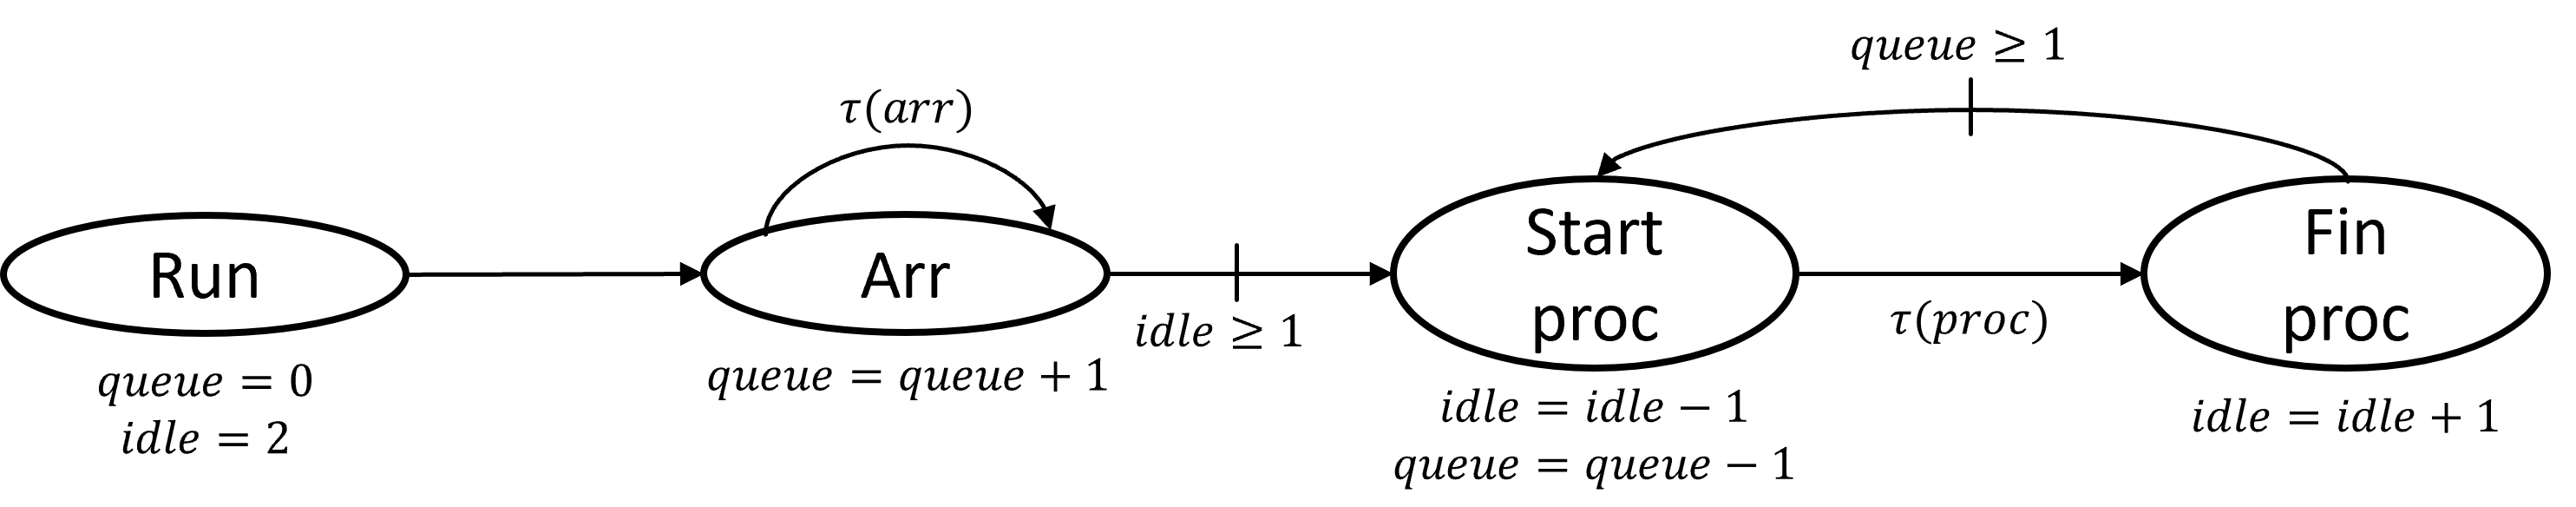
\includegraphics[width=0.8\textwidth]{Figures/GG2-ERG.png}
	\caption{ERG of G/G/2.}
	\label{fig:ERG_GG2}
\end{figure}

The MPR derived from the ERG in Figure \ref{fig:ERG_GG2} is as follows:
\begin{eqnarray}
&  \min {\sum_{i=1}^n (e^{Arr}_i + e^{Start\ proc}_{i} + e^{Finish\ proc}_{i})} \label{erg_1}\\
& e^{Arr}_{i+1} - e^{Arr}_i \ge \tau^{Arr}_{i} &\forall i=1,...,n-1\label{erg_2}\\
& e^{Start\ proc}_{i} - e^{Arr}_i\ge 0 &\forall i=1,...,n\label{erg_3}\\
& e^{Fin\ proc}_{i^{'}} - e^{Start\ proc}_{i} \ge \tau^{proc}_{i} + M (\delta^{Start\ proc, Fin\ proc}_{i,i^{'}} -1)&\forall i=1,...,n\label{erg_4}\\ 
& \sum_{i=1}^{n} \delta^{Start\ proc, Fin\ proc}_{i,i^{'}} = 1 &\forall i^{'}=1,...,n\label{erg_6}\\
& \sum_{i^{'}=1}^{n} \delta^{Start\ proc, Fin\ proc}_{i,i^{'}} = 1 &\forall i=1,...,n\label{erg_7}\\
& e^{Start\ proc}_{i+2} -  e^{Fin\ proc}_{i} \ge 0 &\forall i=1,...,n-2\label{erg_8}\\
& e^{Start\ proc}_{i+1} - e^{Start\ proc}_{i} \ge 0 &\forall i=1,...,n-1\label{erg_9}\\
& e^{Fin\ proc}_{i+1} - e^{Fin\ proc}_{i} \ge 0 &\forall i=1,...,n-1\label{erg_10}\\
& e^{Arr}_i \ge 0, e^{Start\ proc}_{i} \ge 0, e^{Fin\ proc}_{i}\ge 0 &\forall i=1,...,n \label{erg_11} \\
& \delta^{Start proc, Fin proc}_{i,i^{'}} \in \{0,1\}
\end{eqnarray}

The objective function \eqref{erg_1} is the minimization of the execution time of all the events. Constraints \eqref{erg_2} to \eqref{erg_8} are derived from the arcs in the ERG, and indicate the event triggering relationships. The arc pointing from $Arr$ to $Arr$ generates constraints \eqref{erg_2}, which represent the inter-arrival time between two adjacent arrivals. The arc pointing from $Arr$ to $Start\ proc$ generates  constraints \eqref{erg_3}, representing that a job can be processed only after it arrives. The arc pointing from $Start\ proc$ to $Fin\ proc$ generates the constraints \eqref{erg_4} to \eqref{erg_7}, representing that a job can be finished only after the process starts and a certain processing time is elapsed. Since the processing time is generated from probability distributions, it can take different values for different jobs. A job started later can be finished before an earlier stated one, i.e., the ranking of the $i$-th started job in the finishing sequence can be different from $i$. Therefore, binary variables $\delta^{Start\ proc, Fin\ proc}_{i,i^{'}}$ are introduced, and the $i$-th started job is the $i^{'}$-th to finish if and only if $\delta^{Start\ proc, Fin\ proc}_{i,i^{'}}$ is equal to one. The arc pointing from $Fin\ proc$ to $Start\ proc$ generates the constraints \eqref{erg_8}, and represent that a job can be started when there is an idle server. The subscripts $i$ of variables $e^{Start\ proc}_{i}$ and $e^{Fin\ proc}_{i}$ indicates the occurrence sequence of the events, as in constraints \eqref{erg_9} and \eqref{erg_10}. 

This MPR model is different from the one proposed in this work in the following aspects. First, the system states, which are the decision variables in the model proposed in this work, are not explicitly modeled in the Chan and Schruben's model. Second, in the Chan and Schruben's model, the objective is to minimize all the event execution time. Instead, the formulation of objective function can be more flexible in the model proposed in this work, since executing events as soon as possible is already assured by the constraints. Third, \cite{chan2008optimization} only proposed the descriptive procedure to generate an MPR, without well-formulated mapping from ERG to MPR, which makes the application difficult. In this work, instead, the proposed method is well-formulated, and the only required input is the timed Petri net.


\subsection{MPR optimizing the server number of G/G/m queue}
An MP model optimizing the server number in a G/G/m queue, based on the MPR proposed in Section \ref{sec:MPR_ggm}, can be formulated as follows. 
As known, the larger the number of servers, the smaller the waiting time. However, servers have a cost, and this is why their number should be minimized.  
The objective function \eqref{opt_1} is then the minimization of the number of servers, which is the initial marking in place $p^{idle}$, i.e., variable $m^{idle}_0$. However, a constraints must be set on the maximum allowed waiting time, otherwise the obvious solution of number of servers equal to 1 is the one reached by the MPR solution.

\begin{eqnarray}
	&\min{m^{idle}_0} \label{opt_1} \\
	&\sum_{i=1}^{n} (e^{t,f}_i-e^{t,f}_i) \le wt\cdot n \label{opt_2}\\
	&(A1) - (A7),\ (B1) - (B7),\ (C1) - (C4),\ (D1) \nonumber
\end{eqnarray}

Constraint \eqref{opt_2} indicates that the average waiting time does not have to exceed a target value $wt$. Constraints (A1) - (A7), (B1) - (B7), (C1) - (C4), (D1) are the same as presented in Section \ref{sec:MPR_ggm}.

\section{Conclusion} \label{sec:conclude}
This work proposes a well-formulated framework to translate general TPNs into MP models. The convenience of the formulation procedure is demonstrated using the example of a $G/G/m$ queue.

This work lays a common foundation for developing MP--based approaches that can be used to analyze and optimize TPNs, based on the vast literature available in the mathematical programming field. 

In fact, even though many existing works in the literature are related to this research direction, they are mainly focused on specific applications, especially in manufacturing systems, and a methodological work is still %a blank,
mussing, which will be the object of future research development. 

\bibliographystyle{apacite}
\bibliography{RAP, Biblio_Loop}

\end{document}
